\section{Introduction}
\label{sec:intro}
Graphs serve as a natural repository for information in many real-world applications ranging from social, informational, chemical, and biological domains \cite{cho_friendship_2011}. Especially as data becomes more and more unstructured, graphs represent a flexible manner for storing and relating different nodes and their related features \cite{washio_state_2003}. Indeed, graphs represent one of the most general mathematical structures for relating data and are seeing increasing use in modeling phenomenon such as social networks and gene regulatory networks \cite{washio_state_2003,petralia_new_2016}. For the purposes of this work, given a set of vertices $V$, node features $\mathcal{X} : V \rightarrow \mathbb{R}^{d}$, a set of edges $E \subseteq V \times V$, and weights on the edges $W : E \rightarrow [0,1]$, we consider the graph $G = \{V, \mathcal{X}, E, W\}$. Additionally, we let the space of all graphs for a given set of vertices $V$ be $\mathcal{G}$. Below in figure \ref{fig:graph_ex}, a simple visualization of this definition can be seen for a cyclic graph of order 3.
\begin{figure}[b]
  \centering
   \begin{tikzcd}
    & {v_1, \mathcal{X}_1} \arrow[rdd, "{W(v_1, v_2)}"] &                                                   \\
    &                                                   &                                                   \\
    {v_3, \mathcal{X}_3} \arrow[ruu, "{W(v_3, v_1)}"] &                                                   & {v_2, \mathcal{X}_2} \arrow[ll, "{W(v_2, v_3)}"']
  \end{tikzcd}

  \caption{An example graph as related to the terminology laid out \hyperref[sec:intro]{above}}
  \label{fig:graph_ex}
\end{figure}

\subsection{Graph Neural Networks}
To deal with the proliferation of graphs in computing and the need to construct models that consider graphs as a first-class member of the modeling process, a class of models known as Graph Neural Networks have emerged (GNN) with state of the art performance on a variety of classification and regression tasks \cite{ying_gnnexplainer_2019}. Specifically, GNNs and their early iterations in GCNs took inspiration from CNNs that represented applying successive convolution operations on regular grids of information, such as images, to compose local features in the grid in to higher-level predictions \cite{defferrard_convolutional_2017}. At a high level, most GNN frameworks can be split into three steps \verb|MSG|, \verb|AGG|, and \verb|UPD| representing a messaging step, aggregation step, and update step, respectively.

At a layer $l$ in a GNN model $\phi$, the update of the hidden state of the model occurs first by sending messages for all $(v_{i}, v_{j}) \in E$ as a function of the hidden state $\mathcal{H}_{i}^{l-1}$ and $\mathcal{H}_{j}^{l-1}$ as well as the weight $W_{ij} := W(v_{i}, v_{j})$. Specifically, we have
\begin{align*}
  m_{ij}^{l} := \mathtt{MSG}(\mathcal{H}_{i}^{l-1}, \mathcal{H}_{j}^{l-1}, W_{ij})
\end{align*}
Then, a GNN performs an aggregation step wherein it calculates an aggregate message for every vertex $v \in V$. Let $\mathcal{N}_{k} : V \times E \rightarrow \mathcal{P}(E)$ be a function that returns the edges in the $k$-hop neighborhood of a node. Then, we can formally write the aggregation step as
\begin{align*}
  M_{i}^{l} := \mathtt{AGG}(\{m_{ij}^{l} \mid v_{j} \in \mathcal{N}_{k}(v_{i})\})
\end{align*}
Then, finally, at each node, the GNN takes a nonlinear function (often a neural network of some sort) and applies it to this aggregated message $M_{i}^{l}$ along with the hidden state $\mathcal{H}_{i}^{l-1}$ to get the new hidden state.
\begin{align*}
  \mathcal{H}_{i}^{l} := \mathtt{UPD}(\mathcal{H}_{i}^{l-1}, M_{i}^{l})
\end{align*}
When composed in layers, this forms a full Graph Neural Network. Note that in this framework, $\mathcal{H}_{i}^{0} := \mathcal{X}_{i}$. Based on the task type, either node or graph classification in this work, further layers may be added on top of the final output. For example, in graph classification, it is often the case that the final node embeddings are concatenated and then run through an MLP to get a final classification for the whole graph \cite{ying_gnnexplainer_2019}.

The specific layers used in this work are Graph Convolution Layers also known as GCNs \cite{kipf_semi-supervised_2017}. In the context of the framework above, the \verb|MSG| sends weighted and normalized node features from the $l-1$st layer where the normalization is by the out-degree of the sending node and the weight of the message coming from $\mathcal{W}_{ij}$. In the \verb|AGG| step, all of these messages are summed together. Finally, the \verb|UPD| step applies a neural network, usually a trainable linear layer combined with a non-linear activation function to provide a non-linear update step.

\subsection{Interpretation on GNNs}
\label{sec:intro-interp}
Given a GNN, it is natural in many fields such as computational biology to perform interpretation on the model in order to gain further insights. For example, in the case of RNA-seq data, a natural question is to determine important regulatory pathways between genes that could be related to eventual up or down regulation of a target gene \cite{petralia_new_2016}. One natural way to perform this task is to train a GNN on the RNA-seq data for a node-classification task and feed it a large graph $G$ with many redundant edges. Given a GNN model $\phi$ with $l$ layers and a target gene $v_{i} \in V$, we would like to determine $\mathcal{E}_{i} \subseteq \mathcal{N}_{l}(v_{i}, E)$ as well as $\mathcal{W}_{i} : \mathcal{E}_{i} \rightarrow [0,1]$ such that $\mathcal{E}_{i}, \mathcal{W}_{i}$ represent the most important subgraph for the model $\phi$ to perform its predictions for the input vertex $v_{i}$. While there are a few criteria for determining importance, we consider importance to be the maximal mutual information between the original model with its inputs and the same model with the estimated subgraph $\mathcal{E}_{i}, \mathcal{W}_{i}$. Written more formally, we wish to discover
\begin{align*}
  \argmax_{\mathcal{E}_{i}, \mathcal{W}_{i}} \mathtt{MI}(\phi(v_{i}, \mathcal{X}, E, W), \phi(v_{i}, \mathcal{X}, \mathcal{E}_{i}, \mathcal{W}_{i}))
\end{align*}
This is a computationally hard problem as a brute force search would take $O(2^{|E|})$ time even when discounting the weight array $\mathcal{W}_{i}$. In practice, discovering $\mathcal{E}_i$ is ignored and most of the importance discovery is done through learning a suitable $\mathcal{W}_i$ while letting $\mathcal{E}_i = E$.

However, because of the given task, and the various properties we would like to see in a reasonable interpretation of a GNN model, there are many routes that have been taken to interpret these models. As will be shown in \S\ref{sec:related}, there have been a few non-Bayesian attempts to solve this problem. The goal of this work is to analyze these methods and then suggest a new Bayesian method to solving the issue of searching for the best subgraph for a trained GNN to perform post-hoc analysis of importance. Furthermore, an added benefit of utilizing a Bayesian approach is that a full conditional distribution over the importance graph is learned giving researchers an even larger level of insight into their model that goes beyond just a simple edge mask.

\subsection{Bayesian Inference}
Recently, in deep learning literature there has been a rise in utilizing Bayesian methods to create Bayesian Neural Networks in order to provide uncertainty aware predictions \cite{jospin_hands-bayesian_2022}. While primarily concerned with giving estimates for failure modes and reducing overfitting within deep learning methods, the synthesis of Bayesian methods and deep learning models has imbued them with a greater sense of interpretability and introspectability. In the context of GNN interpretation, modeling the subgraph $\mathcal{E}_i, \mathcal{W}_i$ as a joint distribution allows for conditioning on certain edge weights and imbues the interpretations that are derived with a greater sense of introspectability. Figure \ref{fig:bnn_overview} gives a good overview of the deep learning analogues for point estimate neural networks. In the same way, analogues will be utilized in the interpretation task in order to get the same benefits that have already been outlined in BNNs.
\begin{figure}[t]
  \centering
  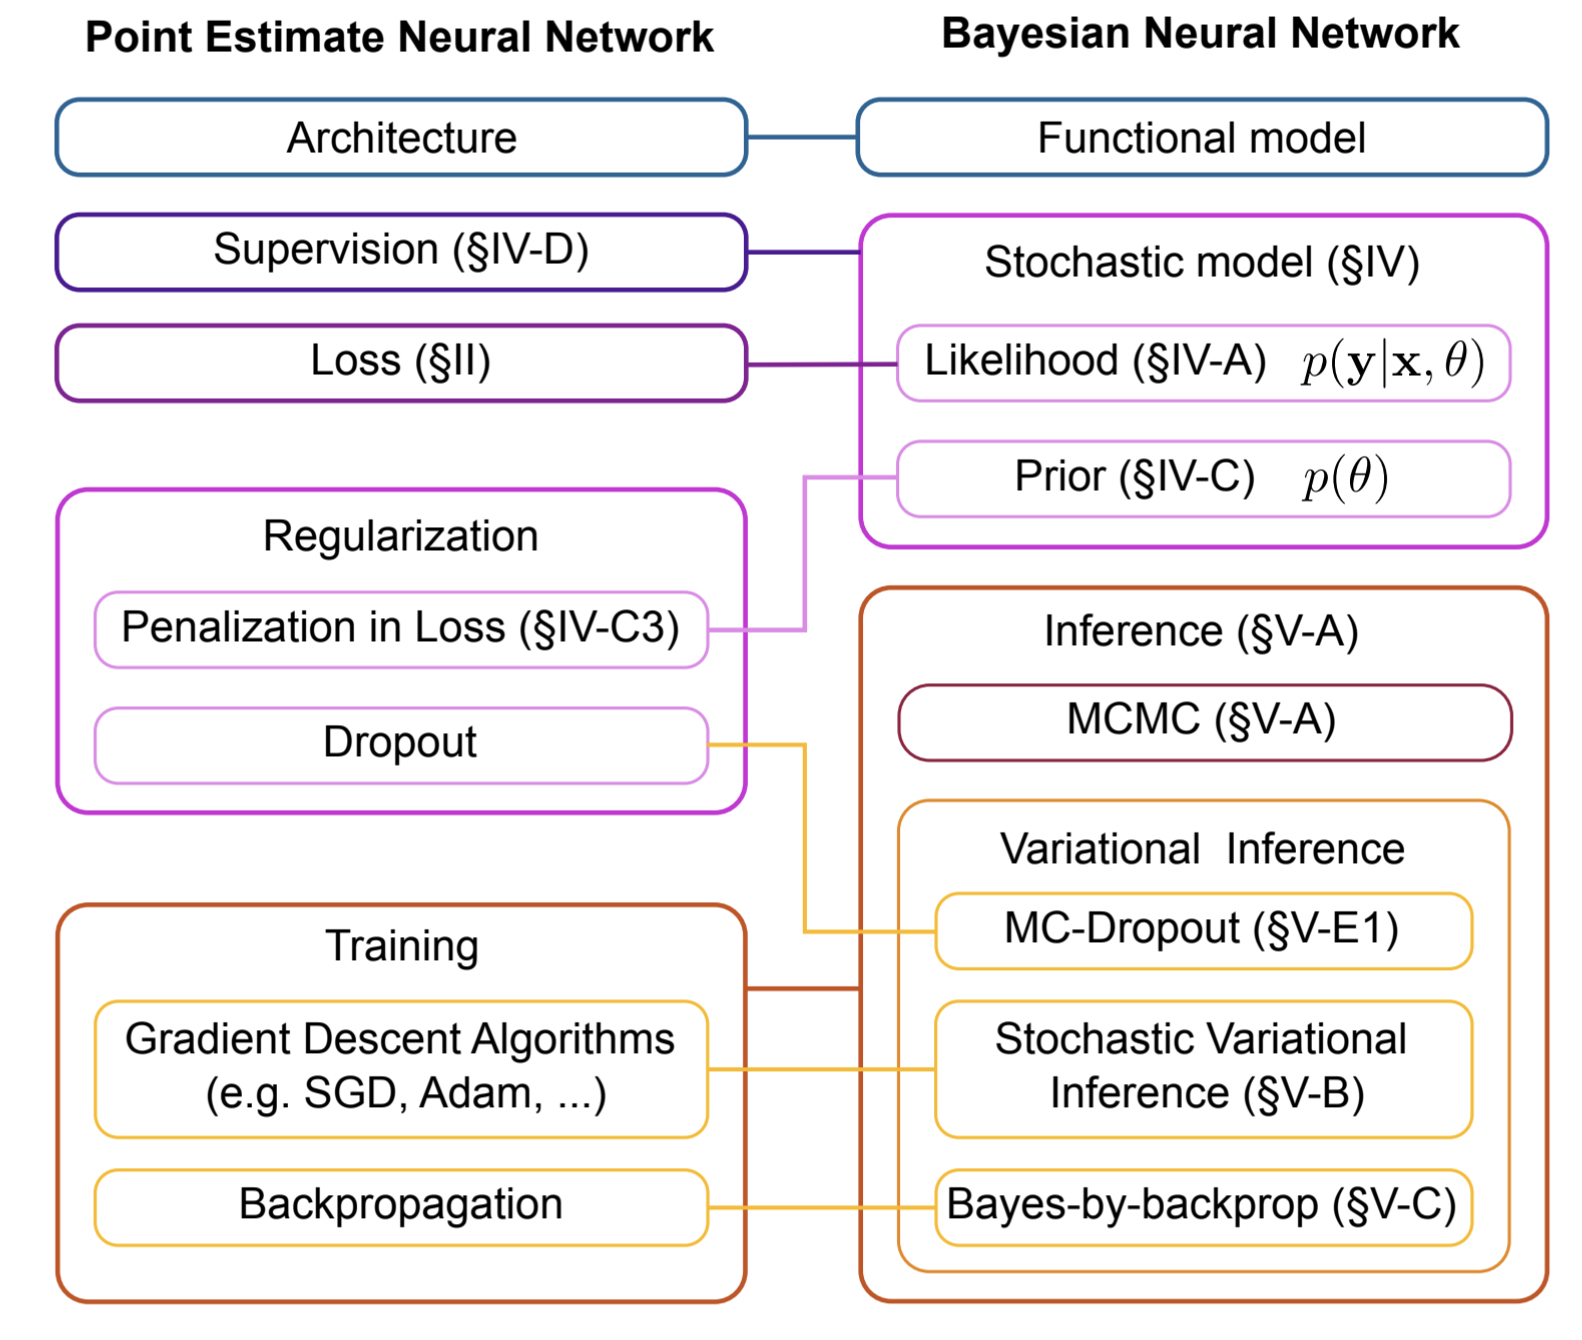
\includegraphics[width=0.9\textwidth]{images/bnn.jpeg}
  \caption{An overview of the corresponding structures in a standard neural network and a Bayesian neural network. Originally appeared in \cite{jospin_hands-bayesian_2022}.}
  \label{fig:bnn_overview}
\end{figure}
In the Bayesian paradigm, a distribution $\mathcal{P}$ is treated as the belief in the occurrence of a given event from the distribution rather than the limit of the frequencies of each event as in the frequentist scheme. Furthermore, prior beliefs are thought to inform posterior beliefs. In the context of interpretability this is important as the belief for a given interpretation is dependent on the domain that it is brought up in. \hyperref[fig:prior]{For example}, in social networks one may expect relatively dense explanations while in biology they would tend to be sparse \cite{cho_friendship_2011} \cite{petralia_new_2016}.
\begin{figure}[t]
  \centering
  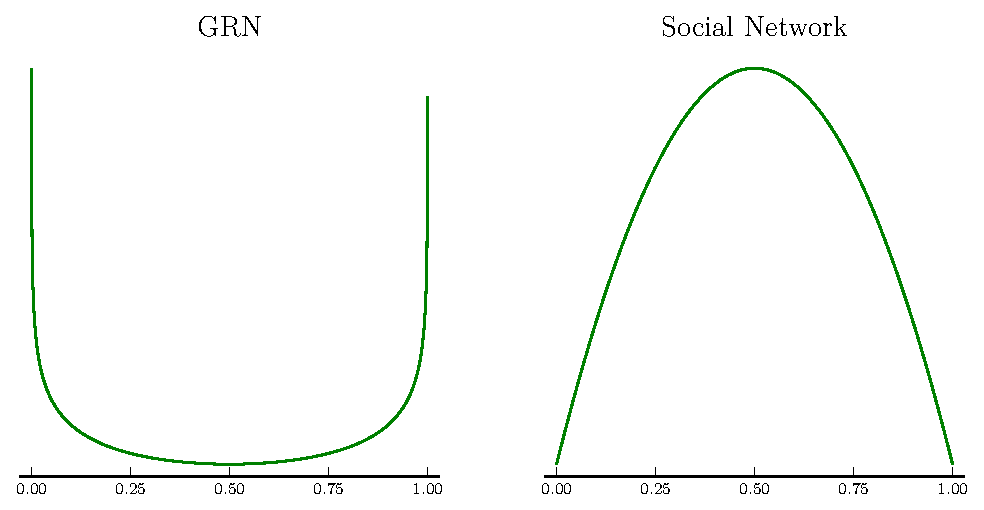
\includegraphics[width=0.95\textwidth]{images/prior.pdf}
  \caption{Idealized prior distributions for GRNs and Social Networks based on the Beta distribution. The displayed distributions are $\Beta(0.95, 0.95)$ and $\Beta(2, 2)$ respectively}
  \label{fig:prior}
\end{figure}
Generally speaking, given a hypothesis $H$ representing the prior belief for the state of a system and some data $D$, the posterior probability $\mathcal{P}(H\mid D)$ can be calculated as
\begin{align*}
  \mathcal{P}(H\mid D) &= \frac{\mathcal{P}(D\mid H)\mathcal{P}(H)}{\mathcal{P}(D)}
\end{align*}
and in this way, the posterior is conditioned by both the prior belief and the evidence that the data presents. While there are a variety of different techniques that can be used to update the prior belief into a posterior distribution as seen in figure \ref{fig:bnn_overview}, in this paper only stochastic variational inference (SVI) and Bayes-by-backprop are utilized. 

\subsubsection{Stochastic Variational Inference (SVI)}
While other inference methods such as MCMC (with popular algorithms including HMC and NUTS \cite{betancourt_conceptual_2018} \cite{hoffman_no-u-turn_2011}), allow exact sampling from the posterior distribution, these methods have proven unpopular with the BNN community due to their algorithmic complexity and lack of scalability to larger models. Hence many communities use SVI which is not an exact method. In SVI, there is a family of distributions $q_{\phi}(H)$ which are parameterized by parameters $\phi$. A common example would be the family of normal distributions parameterized by their mean and covariance structure. The goal of SVI is to approximate the posterior $\mathcal{P}(H \mid D)$ as closely as possible by $q_{\phi}(H)$. The most common measure of approximation in probability space is given by the Kullback-Leibler divergence (KL-divergence). While not a proper metric over the space of distributions, it does give a computationally-reasonable method to optimize against $\phi$ to get as close a match as possible. Specifically, SVI aims to minimize
\begin{align*}
  D_{KL}(q_{\phi} \mid\mid \mathcal{P}) = \int_H q_{\phi}(H')\log \frac{q_{\phi}(H')}{\mathcal{P}(H' \mid D)} dH'
\end{align*} 
This is still problematic since the quantity $\mathcal{P}(H \mid D)$ would still need to be calculated. Hence, it is sufficient to optimize against the ELBO which serves as a lower-bound for the KL-divergence. The ELBO is defined as
\begin{align*}
  \log \mathcal{P}(D) - D_{KL}(q_{\phi} \mid\mid \mathcal{P}) = \int_H q_{\phi}(H')\log \frac{\mathcal{P}(H', D)}{q_{\phi}(H')} dH'
\end{align*}
Note here that $\log \mathcal{P}(D)$ is just a constant meaning that minimizing the KL-divergence is the same as maximizing the ELBO. Note that, generally speaking, the families $q_{\phi}$ tend to come from the exponential family of distributions and the parameters for these families are then just optimized using a typical SGD algorithm such as ADAM \cite{kingma_adam_2017}.

\subsubsection{Bayes-by-backprop}
\label{sec:bayes-by-backprop}
While SVI provides a good framework for Bayesian inference, it does not quite work for deep learning applications because stochasticity stops backpropogation from going through a neural network. To mitigate this problem, the usual reparametrization technique used in creating variational autoencoders (VAEs) \cite{kingma_introduction_2019} is combined with SVI to create a deep-learning friendly SVI algorithm. In this variation, a simple non-parameterized random variable $\epsilon \sim q(\epsilon)$ is sampled. To obtain the family $q_{\phi}(\theta)$, a deterministic transformation $t(\epsilon, \phi)$ is applied such that $\theta = t(\epsilon, \phi)$ has the property that $\theta \sim q_{\phi}(\theta)$. To obtain such a $t$, only a certain class of functions can be utilized. These functions are broadly known as bijectors and require $t$ to be a diffeomorphism. In more detail, let $t : M \rightarrow N$ be a differentiable map, then $t$ is a diffeomorphism if it is a bijection and its inverse $t^{-1} : N \rightarrow M$ is differentiable as well. 

Generally speaking, the exponential family of distributions can all be constructed from such transformations meaning that they are good candidates for Bayes-by-backprop. Note though, that because of the transformation $t$, the formula for the ELBO changes to the following
\begin{align*}
  \int_{\epsilon} q_{\phi}(t(\epsilon, \phi)) \log \frac{\mathcal{P}(t(\epsilon, \phi), D)}{q_{\phi}(t(\epsilon, \phi))}|\text{det}(\nabla_{\epsilon} t(\epsilon, \phi))| d\epsilon
\end{align*}
This is much friendlier to compute since $\epsilon$ is now a constant with respect to $\phi$ and lets us perform SVI through multiple layers of transformations simply by using bijectors like $t$.

\subsection{Normalizing Flows}
\label{sec:normalizing-flows}
The technique that was described in \S\ref{sec:bayes-by-backprop} is more generally known as a normalizing flow. While it was described earlier in the context of a reparametrization technique in which the $t$ are fixed, there is no such restriction in reality. More concretely, the $t$ do not have to be simple functions but, rather, can be learnable functions in their own right. This allows one to use the normalizing flow technique to perform tasks like density estimation and distribution fitting with a very flexible class of transforms that take a simple distribution like a standard multivariate normal and make them into any computable distribution \cite{kobyzev_normalizing_2021}.
\begin{figure}[t]
  \centering
  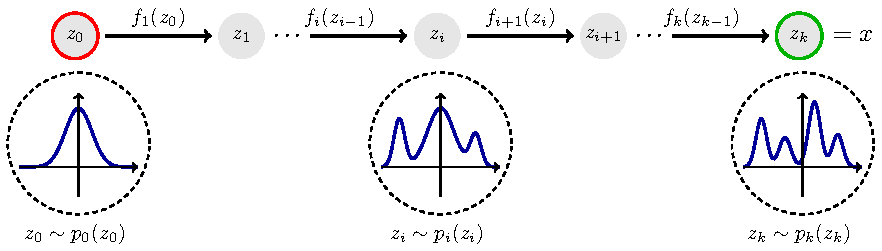
\includegraphics[width=0.9\textwidth]{images/nf.pdf}
  \caption{Chaining learnable bijectors to transform a base distribution to a more complicated distribution from \cite{weng_flow-based_2018}}
  \label{fig:nf}
\end{figure}
Let the transformations of the base distribution be defined as $g = g_n \circ g_{n-1} \circ \dots \circ g_1$ with inverse $f = g_1^{-1} \circ g_2^{-1} \circ \dots g_n^{-1}$. Then we know that the determinant of the Jacobian of $f$ is given by the product of the determinants of the Jacobians at each intermediate evaluation of the flow. This allows for more and more complicated transformations by introducing more and more learnable layers as can be seen in figure \ref{fig:nf}. This structure is very similar to that of an artificial feed-forward neural network. As an example, the simplest form of a normalizing flow is
\begin{align*}
  g_i(x) = Ax + b
\end{align*}
with the learnable parameters here being the matrix $A$ and bias vector $b$. As long as $A$ is an invertible matrix, we have a bijective function that can be used as a normalizing flow layer. Note that these linear layers can be interleaved with activation functions to provide non-linear transformations. This is important as a linear transformation of an exponential family will remain exponential so an element of non-linearity is required (as is the case with MLPs). While RELU is not invertible, a formulation like leaky-RELU can be used for this task \cite{xu_empirical_2015}. Still these are not super expressive. For a normalizing flow with universality, this paper utilizes rational quadratic spline based flows \cite{durkan_neural_2019}. When combined with variational inference over the prior base-distribution, this allows for a very flexible estimation of the posterior distribution no matter how complex.
\newpage
